%%!TEX root = main.tex
\section{Discussion}


% \begin{figure}[t]
% 	\centering
%     \footnotesize
%     \setlength{\tabcolsep}{1pt}
%     \begin{tabular}{cccc}
%     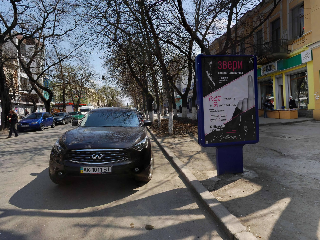
\includegraphics[width=.24\linewidth]{figures/nn_interest_region_visualization/pano_arkbipzrfswzce-0.png} & 
%     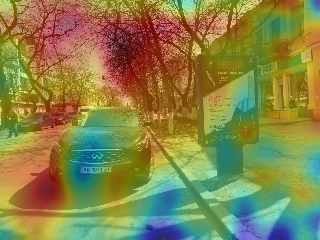
\includegraphics[width=.24\linewidth]{figures/nn_interest_region_visualization/pano_arkbipzrfswzce-0-overlay.png} & 
%     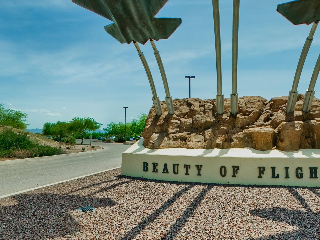
\includegraphics[width=.24\linewidth]{figures/nn_interest_region_visualization/pano_albijadjmaqlft-0.png} & 
%     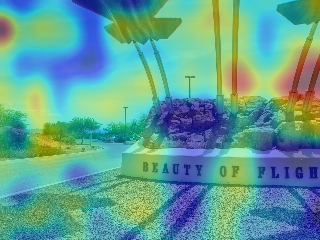
\includegraphics[width=.24\linewidth]{figures/nn_interest_region_visualization/pano_albijadjmaqlft-0-overlay.png} \\
%     \multicolumn{2}{c}{(a)} & \multicolumn{2}{c}{(b)} \\
%     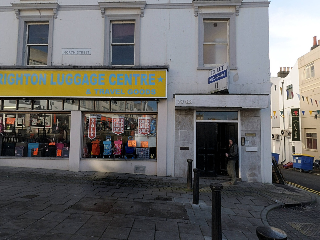
\includegraphics[width=.24\linewidth]{figures/nn_interest_region_visualization/pano_aigrekyvbnoxlg-5.png} & 
%     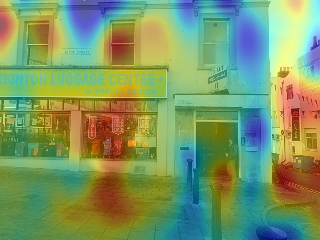
\includegraphics[width=.24\linewidth]{figures/nn_interest_region_visualization/pano_aigrekyvbnoxlg-5-overlay.png} & 
%     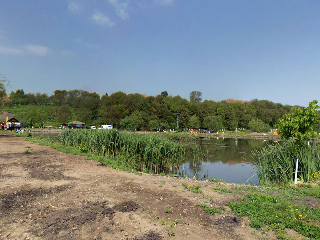
\includegraphics[width=.24\linewidth]{figures/nn_interest_region_visualization/pano_agolqlvjxtuybt-1.png} & 
%     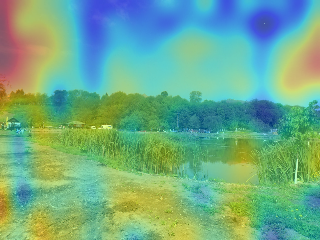
\includegraphics[width=.24\linewidth]{figures/nn_interest_region_visualization/pano_agolqlvjxtuybt-1-overlay.png} \\
%     \multicolumn{2}{c}{(c)} & \multicolumn{2}{c}{(d)} \\
%     \end{tabular}
%     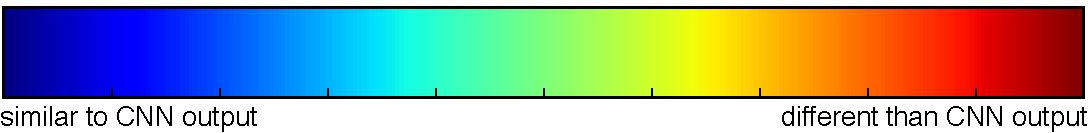
\includegraphics[width=.5\linewidth]{figures/nn_interest_region_visualization/colorbar-tags.pdf}
% 	\caption{What is the network looking at when predicting the sun position? By forwarding a sweeping $60\times60$ window to the CNN and setting every pixel outside to 0, we compute the L1 distance between the network output with the windowed input compared to its response using the original image. A region with a low L1 distance (blue) indicates a sun position estimation closer to the output obtained when the full image is shown to the network. This analysis suggests that the network is sensitive to specific cues like shadows (a) and (b), shading (c), and sky gradients (d).}
% 	\label{fig:attention-analysis}
% \end{figure}

% The proposed method estimates accurately the sun position as well as sky and camera parameters from a single outdoor LDR image. A CNN is employed at its core to produce the estimations directly from the image. While previous art relies mostly on hand-crafted features, the proposed method provides an end-to-end training approach which automatically learns the features it needs to perform its task. Understanding the features learned by the CNN is a hard task in itself, it is however possible to figure out the regions of the image that the neural network relies on to achieve its estimations. By showing a single region of an input image, it is possible to measure how its estimations are varying~\ref{fig:attention-analysis}.

%the approach we proposed does not produce occlusion masks. Objects occluding the sky and/or the sun are currently not modeled and may yield wrong results when the sun is .

In this chapter, we propose what we believe to be the first end-to-end approach to automatically predict full HDR lighting models from a single outdoor LDR image of a general scene, which can readily be used for image-based lighting. Our key idea is to train a deep CNN on pairs of photos and panoramas in the SUN360 database, which we ``augment'' with HDR information via a physics-based model of the sky. We show that our method significantly outperforms previous work, and that it can be used to realistically insert virtual objects into photos.

Despite offering state-of-the-art performance, our method still suffers from some limitations. First, the Ho\v{s}ek-Wilkie sky model provides accurate representational accuracy for clear skies, but its accuracy degrades when cloud cover increases as the turbidity $t$ is not enough to model completely overcast situations as accurately as for clear skies. Optimizing its parameters on overcast panoramas often underestimates the turbidity, resulting in a bias toward low turbidity in the CNN. We are currently investigating ways of mitigating this issue by combining the HW model with another sky model, better-suited for overcast skies. Another limitation is that the resulting environment map models the sky hemisphere only. While this does not affect much diffuse objects such as the bunny model used in this work, it would be more problematic for rendering specular materials, as none of the scene texture would be reflected off its surface. It is likely that simple material adjustments adding interactions with the scene such as~\cite{khan-siggraph-06} could be helpful in making those renders more realistic. 

